\chapter{数据分析与处理}\label{chap:data}
本论文以天津肿瘤医院的721位病例图片数据为基础,其中包含304例恶性病例,417例正常病例;图片数有2908张,其中包含恶性图片数据有1254张,正常图片数据有1654张。医学数据存在恶性和正常两大分类,对于恶性数据医生容易标注出具体的癌变病灶位置,对于正常样本,包括拥有疑似恶性病灶的良性数据医生难以精确标出,这使得基于深度学习的模型设计存在一定的难度。每个病例数据大多拥有两个乳房不同角度的图片,这使得实际应用中应当考虑标准方面的设计。

\section{数据分析}
\subsection{医学数据分析}
既往我国大多是医疗机构均采用纸质文件记录医疗数据及医疗活动,这些纸质文件数据属于非结构化数据,利用起来非常困难,虽然早就有巨大的数据量,但无法利用。近年来,我国卫生行政部门大力推进以健康档案、电子病历和公共服务信息平台为基础的区域卫生信息化建设工作。2010年“十二五”卫生信息化建设工程规划编制工作初步确定了我国卫生信息化建设路线图。随着卫生信息化建设的不断成熟,医疗相关的大数据也在急剧增加。医院信息管理系统(HIS),主要包括电子病历信息系统(医嘱、病程记录、护理记录等)、实验室信息管理系统(检验报告)、医学影像系统(各种医学影像如MRI、CT、X光片等),这些系统几乎每分每秒都在产生电子化数据,数据量实在是太大、增长太快,数据量从MB到GB,从TB 到PB,对数据处理的实时性、有效性提出更高要求,传统的分析技术无法应付。医学的数据常常是海量的,格式丰富多样,为深度学习的训练提供了有效的数据来源。

另一方面,在传统模式下,数据多数是由不同的应用程序搜集到的,存储格式不一,无法彼此兼容、无法整合,各个数据库就像一个个相互隔离的岛屿,由此产生了“数据孤岛”的概念。比如我国人口死亡登记系统实际上保存着大量的、相对准确的人口死亡信息,包括死亡日期和死亡原因等,这些数据对于评价临床医疗结局无疑是宝贵的原始资料。但是由于各种原因,这部分数据与医院的医疗方面的数据至今无法整合,令人惋惜。再加上存在着不同的地方存在着器官组织的差异,比如乳腺腺体,东方女性偏致密性,所以基于医学数据的项目在中国目前大部分只能分别考虑,基于东方女性特点的乳腺钼靶分类就变得很有实际意义,而且对模型的可拓展性也提出了较高的要求。

医疗影像数据一般尺度大,以乳腺钼靶为例,尺度可以达到2000-4000像素左右,而且格式丰富多样,有包括病人各种信息的dicom格式,有包括一个病人多个切片拍摄的CT数据等等,所要识别的目标,无论是器官还是肿瘤病灶一般较小。在所有的数据里,影像的数据跟临床病理比较起来,它的标准化、格式化、统一性是最强的。在图像领域,传统的自然图像一般尺度小,所要识别分类的目标一般较大而且目标与目标之间区别较大,即使属于细粒度分类检测问题,细粒度目标之间的差异也是可以通过肉眼进行区分,而在医疗影像数据中类别之间的差异并不明显。在肿瘤识别中,医学数据常分为阴性,良性和恶性三种类型,其中阴性是不包含任何疑似肿瘤病灶的特征,良性包含疑似恶性肿瘤的信息,而恶性包含恶性肿瘤病灶。基于此,医学会提出各种经验性的指标判断一个病人是否得癌,然后基于病理报告进一步确诊。肿瘤的形态,大小,分布往往各异,不具有统计学上的特征,良性肿瘤和恶性肿瘤之间的差别往往只是在于边缘的细微区别,如何有效的识别并区分这细小的不同便成为医学以及深度学习模型得以学习的关键。同时特别不一样的是,影像数据很难像语音数据或者文本数据一样将标注任务外包出去,影像数据的标注大部分只能依靠专业人士,这使得数据的采集在医疗影像问题上变得难度极大,数据量往往较少也成为制约模型能否具有鲁棒性的关键。

	对于医生而言,医学数据的指标往往更加关注敏感度,特异度等指标。敏感度(sensitivity,SEN):又称真阳性率(true positive rate,TPR),即实际患病又被诊断标准正确地诊断出来的百分比。特异度是实际无病按该诊断标准被正确地判为无病的百分比。 特异度(specificity,SPE),又称真阴性率(true negative rate,TNR),即它反映筛检试验确定非病人的能力。对于医生而言,医生希望在保证不过高的误诊率的基础上,能够降低病人的误诊率。医生考虑的层面和计算机视觉也有所不同,如果一个病人拥有多种不同格式以及在不同时间段采集的数据,他们更关心在病人层面判断该病人是否得癌,是否需要进行手术,是否需要做下一步的病理分析等,进而基于实际情况出发,会影响到基于医学数据的深度学习模型的标准制定。
	
	综上,在医学数据分析的基础上,使用深度学习技术,往往包括以下流程,第一步,对医疗影像数据标注从而获取模型训练所需要的数据资源;
第二步,选择合适的模型对数据进行训练,进而对模型进行测试,反馈测试结果给训练模型,对模型进行调参,优化模型;第三步,在模型测试反馈测试结果的同时,也反馈数据标注的问题,进一步优化数据;第四步,基于实际出发,设计相应的合适指标,对模型进行评估,如果最终需要产业化的话,还需要落地模型,对产品评估等。如图\ref{fig:data_flow}。

	\begin{figure}[!htbp]
    \centering
    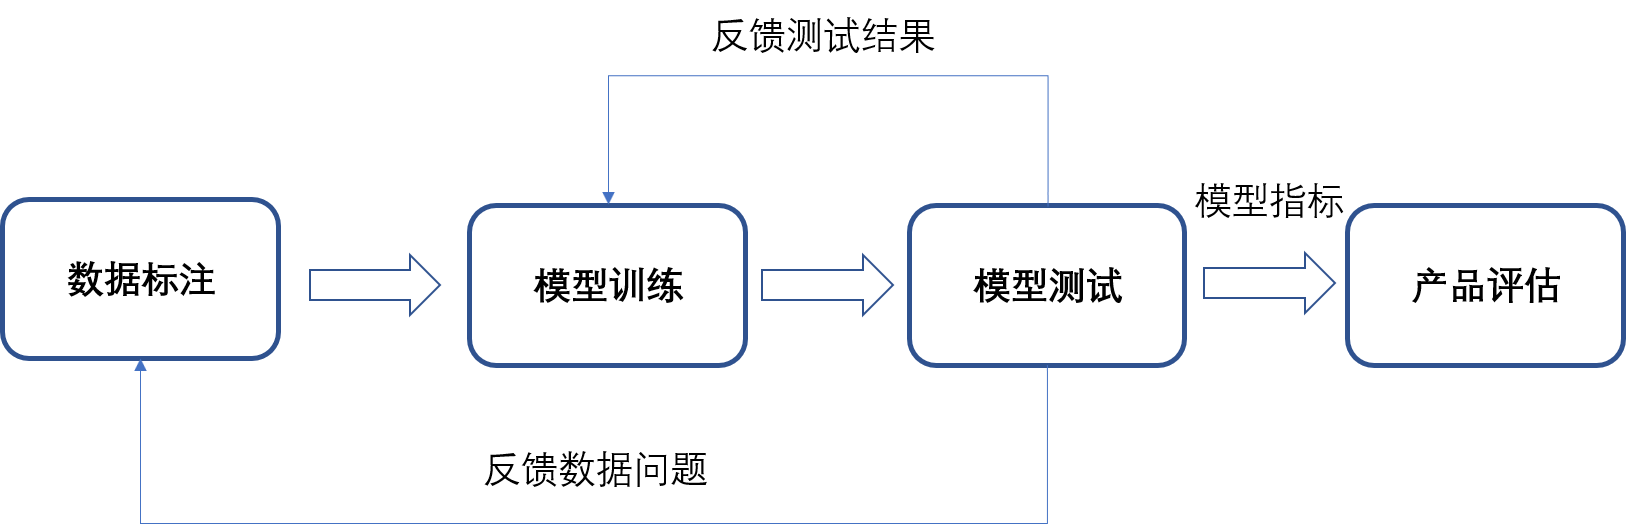
\includegraphics[width=0.7\textwidth]{data_flow}
    \bicaption{基于深度学习的医学数据工作流程}{Medical data workflow based on deep learning}
    \label{fig:data_flow}
	\end{figure}
在上述流程中,数据标注的制定标准,数据本身的特性以及模型指标的确定都是医学数据进行深度学习技术实践中区别于传统的自然图像的地方。在医学影像数据中,尤其需要对数据进行充分的认识,只有对数据标注提出适应于数据的标注要求及模型评估指标,才可以充分的发挥深度学习的作用,更好地服务于实际情况。

\subsection{乳腺钼靶数据分析}
女性在现在的生活工作中担负起了越来越重要的角色,相应的生活工作压力也随之而来,与此同时疾病也不请自来。乳腺癌是女性最常见的浸润性癌症,也是仅次于肺癌的女性癌症死亡的第二大凶手。女性乳腺是由皮肤、纤维组织、乳腺腺体和脂肪组成的,乳腺癌是发生在乳腺腺上皮组织的恶性肿瘤。乳腺癌中99\%发生在女性,男性仅占1\%。目前乳腺癌已成为威胁女性身心健康的常见肿瘤。全球乳腺癌发病率自20世纪70年代末开始一直呈上升趋势。美国8名妇女一生中就会有1人患乳腺癌。中国不是乳腺癌的高发国家,但不宜乐观,近年我国乳腺癌发病率的增长速度却高出高发国家1~2个百分点。据国家癌症中心和卫生部疾病预防控制局2012年公布的2009年乳腺癌发病数据显示,全国肿瘤登记地区乳腺癌发病率位居女性恶性肿瘤的第1位,女性乳腺癌发病率(粗率)全国合计为42.55/10万,城市为51.91/10万,农村为23.12/10万。乳腺癌已成为当前社会的重大公共卫生问题。

自20世纪90年代全球乳腺癌死亡率呈现出下降趋势。究其原因,一是乳腺癌筛查工作的开展,使早期病例的比例增加;二是乳腺癌综合治疗的开展,提高了疗效。乳腺钼靶,全称乳腺钼靶X线摄影检查,又称钼钯检查,是目前诊断乳腺疾病的首选和最简便、最可靠的无创性检测手段,痛苦相对较小,简便易行,且分辨率高,重复性好,留取的图像可供前后对比,不受年龄、体形的限制,目前已作为常规的检查。乳腺钼靶以dicom格式进行保存,dicom全称是医学数字图像与通讯,其文件结构如图\ref{fig:data_dicom}所示。
	\begin{figure}[!htbp]
    \centering
    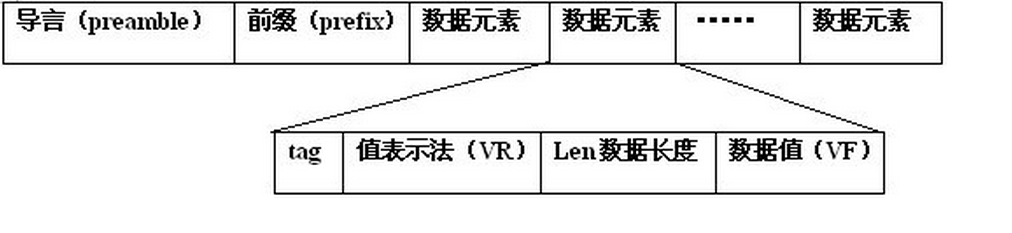
\includegraphics[width=1.0\textwidth]{data_dicom}
    \bicaption{dicom数据格式}{dicom data format}
    \label{fig:data_dicom}
	\end{figure}
dicom整体结构先是128字节所谓的导言部分,接着就是四个字节组成的字符串,然后是数据元素(dataElement)依次排列到文件结尾.我们要读取dicom里面的各种数据就是在各个数据元素中。通俗的讲dataElement就是指tag,就是dicom标准里定义的数据字典,每个dataElement中的tag决定自身或整个文件的某些数据类型或自身dataElement内容类别,从前到后按tag又可简单分类为:文件元tag(定义了传输语法),普通tag(包括图像宽,高,数据传输格式,病人姓名等基本信息),像素tag(表示dataElement存储的是病例的图像数据)。dicom中存储的信息量丰富,对于本文而言,重点关注的是乳腺钼靶的图像数据,也就是像素tag。
通过对乳腺钼靶dicom数据的分析,我们发现乳腺钼靶数据有以下几个特点:

\begin{itemize}
	\item 医疗影像数据采集困难,使得数据集小
	
	以公开的几个数据集为例,INBREAST\cite{27moreira2012inbreast}有116个病例,410张乳腺钼靶图
片;而另一个比较大的乳腺钼靶公开数据集DDSM\cite{21lee2018curated, 22lee2017curated,23clark2013cancer}也只有2620个病例,而且由于年代久远,缺乏维护,其中很多病例数据缺失;我们所采集的天津肿瘤医院的数据,耗时医生半年多时间,最终才采集721个病例,由此可见医疗影像数据多么宝贵。正因为数据集小,所以对我们的模型训练提出更高的要求,因为深度学习得以发展的一个重要因素正是巨大的数据量。

	\item 尺寸大,平均有4000×2000像素,但病灶占比小,如图\ref{fig:data_mam_with_annotation}所示
		\begin{figure}[!htbp]
    \centering
    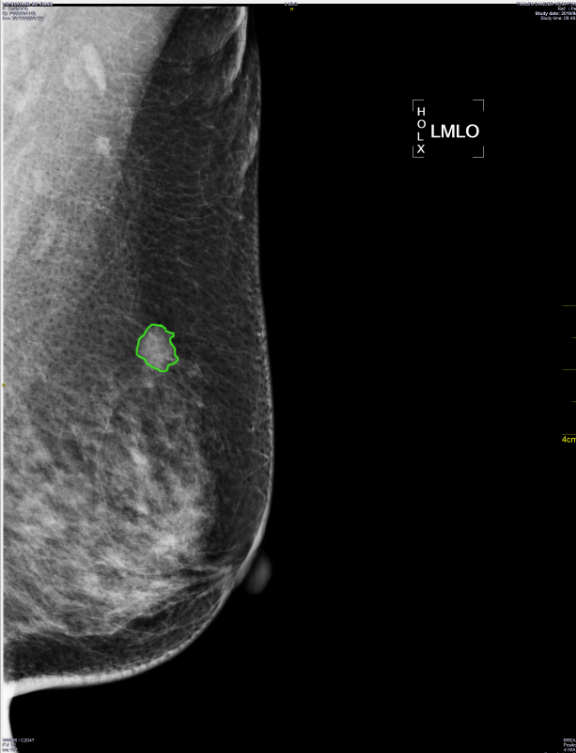
\includegraphics[width=0.6\textwidth]{data_mam_with_annotation}
    \bicaption{带标注信息的乳腺钼靶图片}{Mammography with annotation}
    \label{fig:data_mam_with_annotation}
	\end{figure}
	
	ImageNet图像尺寸主要为299×299像素,乳腺钼靶尺寸大约是传统自然图像像素的十倍,尺度高,训练的维度高,如果直接载入模型,将导致资源消耗高。ImageNet需识别物体占据图像的70\%-80\%。以我们本文的乳腺钼靶数据为例,其中乳腺钼靶图片尺度为3328×2560像素,对乳腺钼靶检测的病灶宽度以高度进行直方图统计,如图\ref{fig:data_hist},所要识别的病灶占比不到2\%。

\begin{comment}
\begin{figure}[htbp]
    \centering
    \begin{subfigure}[a]{0.5\textwidth}
      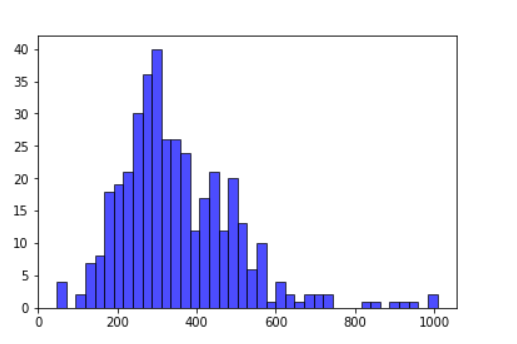
\includegraphics[width=\textwidth]{data_width_hist}
      \caption{}
      \label{fig:data_width_hist}
    \end{subfigure}%
    \qquad
    ~% add desired spacing
    \begin{subfigure}[b]{0.5\textwidth}
      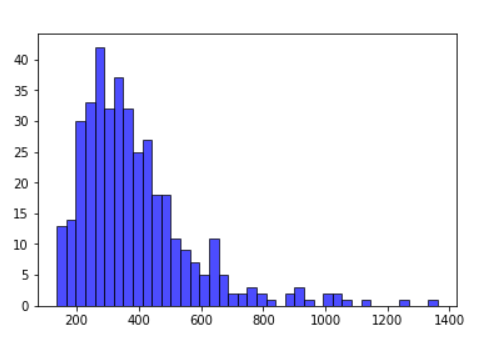
\includegraphics[width=\textwidth]{data_height_hist}
      \caption{}
      \label{fig:data_height_hist}
    \end{subfigure}

    \bicaption{本文乳腺钼靶病灶宽高长度直方图(a) 病灶宽度直方图(b) 病灶高度直方图}{The broad and high length histogram of mammography lesions in this project (a) histogram of lesion width (b) height histogram of lesion}
    \label{fig:data_hist}
\end{figure}
\end{comment}
		\begin{figure}[!htbp]
    \centering
    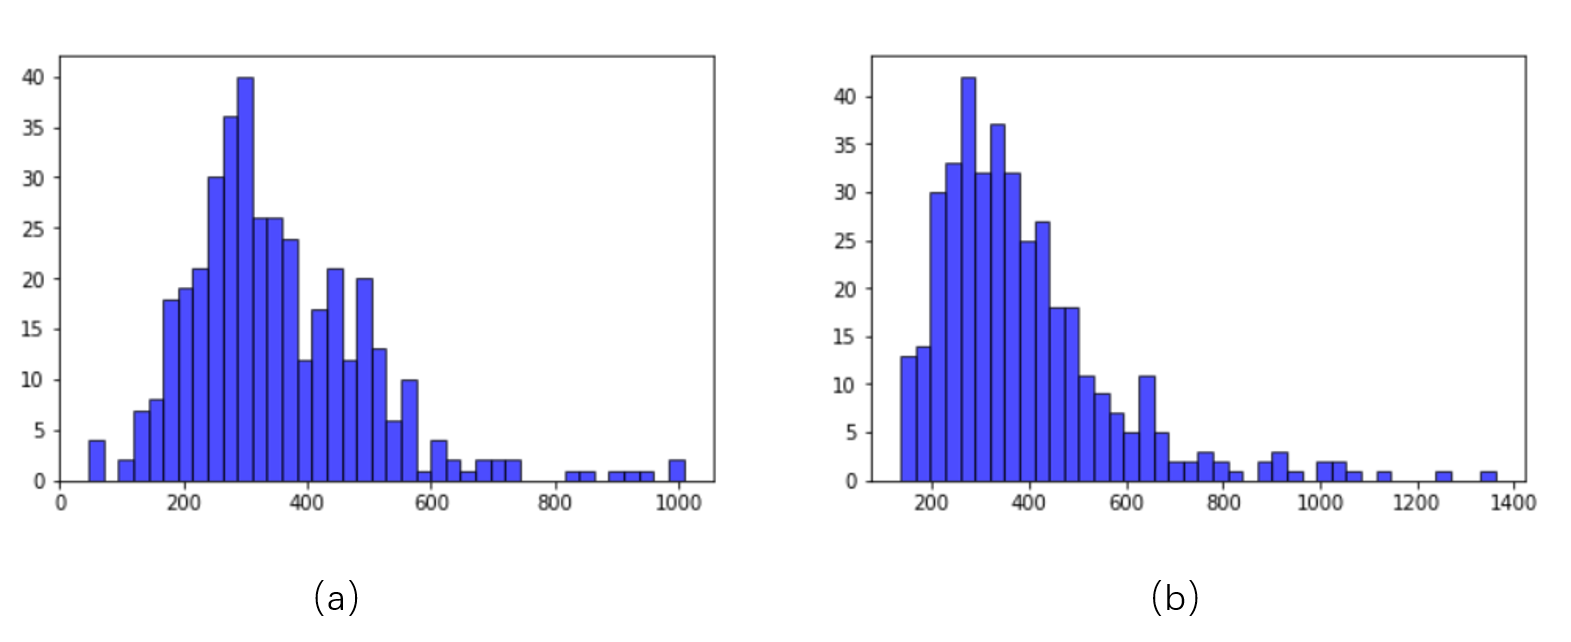
\includegraphics[width=0.6\textwidth]{data_hist}
    \bicaption{本文乳腺钼靶病灶宽高长度直方图(a) 病灶宽度直方图(b) 病灶高度直方图}{The broad and high length histogram of mammography lesions in this project (a) histogram of lesion width (b) height histogram of lesion}
    \label{fig:data_hist}
	\end{figure}
	
	\item 图片分为良性,恶性及阴性
	
	由于所要考量的问题是肿瘤识别问题,所以图片有良性,恶性和阴
性三种类型。按照医学以及实际情况出发,良性和阴性问题常常被判断为正常标签,与恶性标签区分。

	\item 正常数据未标注
	
	由于数据工作量大,而且对于良性中疑似恶性病灶的标注困难,所以正常样本并未标注。

	\item 拥有图片,乳房及病人多层次考虑问题
	
	乳腺钼靶设备会对女性乳腺进行左右乳各个角度的拍摄,如图\ref{fig:data_mam}。
				\begin{figure}[!htbp]
    \centering
    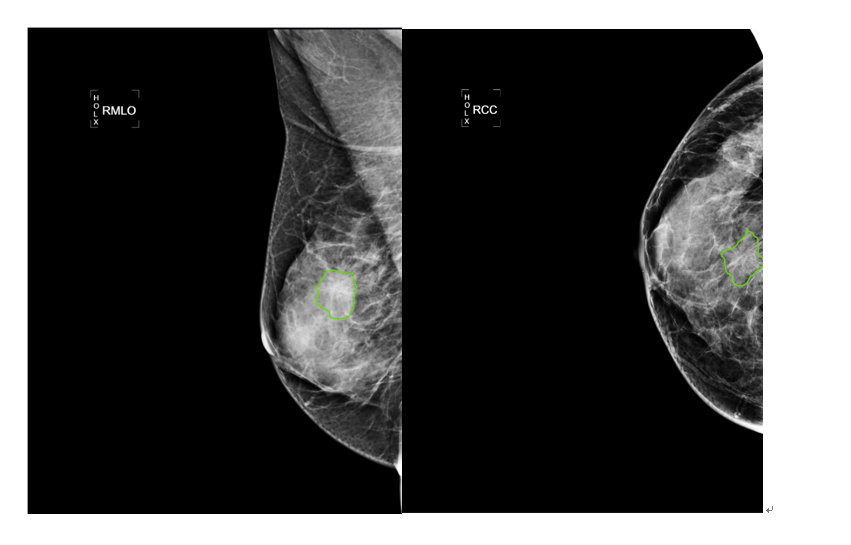
\includegraphics[width=0.6\textwidth]{data_mam}
    \bicaption{同一女性同一乳房不同角度拍摄图片}{The same woman takes pictures of the same breast at different angles}
    \label{fig:data_mam}
	\end{figure}
	
	在医学上,常用MLO及CC作为典型图片进行考量。传统的计算机视觉是以单张图片作为考量层次,而医学上更多关心的是基于单个乳房或者单个病人,在我们这个项目中,更多考虑的是病人是否患癌。这两个不同角度拍摄的图片可以决定一个病人的单一乳房是否得癌,只要有一侧乳房得癌,该病人就得癌。一个得癌病人并不是拍摄的所有角度乳房都会有恶性病灶。
	
	\item 正常样本中包含恶性样本信息
	
	如图\ref{fig:data_all}所示,正常样本中,比如右边两张正常样本(良性和阴性)图片中存在着疑似第一张恶性样本带实线的恶性病灶信息(图中用虚线表示)。
	\begin{figure}[!htbp]
    \centering
    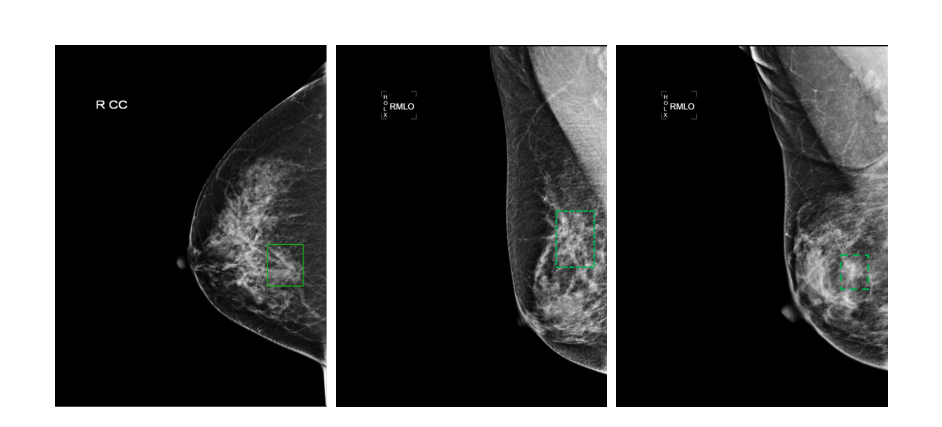
\includegraphics[width=1.0\textwidth]{data_all}
    \bicaption{带有标注框的正样本及包含疑似恶性病灶的正常样本}{
The image with labeled malignant lesion(left) and healthy images contain un-annotated benign tumor region (middle)  or normal region(right) which are suspect to be malignant in vision}
    \label{fig:data_all}
	\end{figure}
	
	
\end{itemize}

\section{数据处理}
\subsection{数据预处理}
在数据预处理方面,我们依次进行了以下的工作:

\begin{itemize}
	\item 去除噪声数据,获取图片的标注框文件。
	\item 转换医学dicom文件格式为jpg格式,进行灰度值变换,使得像素点最终落在0-255之间,拥有RGB三通道,以满足深度学习迁移学习的基本要求。
	\item 原图片尺寸过大,影响训练效率,实际过程中将图片resize到512×512进行训练。
	\item 计算训练集数据的均值,标准差等统计信息;对图片进行可视化查看,确定模型中的具体参数设置,如anchors的尺寸scale,anchors的长宽比aspect ratio等。
	\item 对图片进行零值归一化,计算图片的各通道的均值及标准差,得到三通道的均值为mean=(0.494, 0.494, 0.494),标准差为std=(0.101,  0.101,  0.101)并按照channel=(channel-mean)/std对各通道中的各个像素值归一化到[-1, 1]。
\end{itemize}

\subsection{数据集划分}
总病例个数721例,其中恶性病例304例,良性+阴性(正常)病例417例,总共图片数有2908张,其中有598张带有恶性标注框的恶性图片。

以病例为单位,对病例数进行4:1划分为训练集合测试集,划分后的数据分布如表\ref{tab:data_set_split}所示。最后所要训练的图片个数有2336张,恶性图片1010张,良性+阴性(正常)图片1326张;所要测试的图片个数有572张,恶性图片有244张,良性+阴性(正常)图片328张。对于恶性病例下的图片,并不都是包含标注框,也就是病人体现为恶性并不都是所有乳房拍的所有角度都体现为恶性,所以训练集恶性病例下图片有标注框的只有478张,测试集下则为120张。此时再看训练集数目,带有标注的恶性图片数为478张,训练集中共有2336张图片,使得恶性及良性图片之间存在着大约1:3的不均衡的数据比例,这需要我们为后期的数据处理进行相应的考量。

\begin{table}[!htbp]
	\bicaption{天肿数据集划分}{tianzhong data set partition}
    \label{tab:data_set_split}
    \centering
    \footnotesize% fontsize
    \setlength{\tabcolsep}{4pt}% column separation
    \renewcommand{\arraystretch}{1.2}%row space 
    \begin{tabular}{c|c|c|c|c|c}
        \hline       
         &恶性 &正常 &恶性 &正常 &带有标注的恶性\\
        \hline
        训练集 &244 &334 &1010 &1326 &478 \\
        \hline
        测试集 &60 &83 &244 &328 &120\\
        \hline
    \end{tabular}
\end{table}

\begin{comment}
\begin{table}[!htbp]
	\bicaption{天肿数据集划分}{tianzhong data set partition}
    \label{tab:data_set_split}
    \centering
    \footnotesize% fontsize
    \setlength{\tabcolsep}{4pt}% column separation
    \renewcommand{\arraystretch}{1.2}%row space 
    \begin{tabular}{c|c|c|c|c|c}
        \hline       
        \multirow{2}{*}{} & \multicolumn{2}{|c|}{病例数} & \multicolumn{3}{c}{图片数}\\
        \cline{2-6}
         &恶性病例数 &正常病例数 &恶性图片数 &正常图片数 &带有标注的恶性图片数\\
        \hline
        训练集 &244 &334 &1010 &1326 &478 \\
        \hline
        测试集 &60 &83 &244 &328 &120\\
        \hline
    \end{tabular}
\end{table}
\end{comment}
\begin{comment}
\begin{table}[!htbp]
    \bicaption{数据集划分}{Data set partition}
    \label{tab:data_set_split}
    \centering
    \footnotesize% fontsize
    \setlength{\tabcolsep}{4pt}% column separation
    \renewcommand{\arraystretch}{1.2}%row space 
    \begin{tabular}{ccc}
        \hline
        数据集& 病例数:恶性病例数+正常病例数& 图片数:恶性病例图片数(标注框)+正常病例图片数\\
        \hline
        训练集& 578:244 + 334& 2336:1010(478)+1326\\
		测试集& 143:60 + 83& 572:244(120)+328\\
        \hline
    \end{tabular}
\end{table}
\end{comment}

\section{标准制定}
\subsection{数据定义}
我们将恶性乳腺钼靶定义为正样本(positive),其拥有恶性病灶,所有其他的乳房乳腺钼靶定义为负样本(negative),包括阴性和良性乳腺钼靶,其中良性乳腺钼靶中包含高度疑似恶性病灶的信息。在我们使用的数据集中,所有positive都有标注框表示其精确位置,所有negative没有任何标注信息。

针对乳腺钼靶数据特点以及医院的实际情况,我们设定了两个标准。

\subsection{基于病例}
本研究针对的是乳腺癌中肿块型病变,浸润性导管癌的检测。乳腺钼靶图像尺寸大,平均有4000×2000像素,但病灶占比小;医学上图片经常有良性,恶性和阴性三种类型,其中良性为含有良性肿块的乳腺,恶性为有恶性肿瘤的乳腺,阴性为不存在肿块的乳腺。综合医学和计算机的特点,positive为1,negative为0,我们的问题变成两分类问题。

根据实际需求标准,医生希望在病例层面对结果进行分析,也就是该病例下存在至少一张图片为恶性即可即为恶性,该病例下所有图片均为良性该病例才是良性。基于此,我们引入了多示例学习(MIL)\cite{34Dietterich1997Solving}中关于评判标准的定义。多示例学习可以被描述为:假设训练数据集中的每个数据是一个包(Bag),每个包都是一个示例(instance)的集合,每个包都有一个训练标记,而包中的示例是没有标记的;如果包中至少存在一个正标记的示例,则包被赋予正标记;而对于一个有负标记的包,其中所有的示例均为负标记。(这里说包中的示例没有标记,而后面又说包中至少存在一个正标记的示例时包为正标记包,是相对训练而言的,也就是说训练的时候是没有给示例标记的,只是给了包的标记,但是示例的标记是确实存在的,存在正负示例来判断正负类别)。通过定义可以看出,与监督学习相比,多示例学习数据集中的样本示例的标记是未知的,而监督学习的训练样本集中,每个示例都有一个一已知的标记;与非监督学习相比,多示例学习仅仅只有包的标记是已知的,而非监督学习样本所有示例均没有标记。

针对该医学问题,基于病例情况下,假设我们训练的病例集为$R$,每个病例包含多张乳腺钼靶图片及其标签$\left\{\left(X_{\mathrm{i}}, Y_{\mathrm{i}}\right)\right\}_{i=1}^{N}$,其中$N$表示病例个数,$X_{\mathrm{i}}=\left\{x_{i j}\right\}_{j=1}^{m_{i}}$表示第$i-th$个病例, $x_{i j}$表示第$i-th$病例的第$j-th$张乳腺钼靶图片,对应的预测值为$y_{i j}$,最后对病例预测的值$y_{j}$为:
\begin{equation}
	y_{i j}=\max _{k}\left(y_{i j k}\right)
\end{equation}

其中$k$为预测框的个数,至此,所要求的基于病例预测的值为:
\begin{equation}
	\mathrm{y}_{i}=\max _{j}\left(\left(\max _{k}\left(y_{i j k}\right)\right)\right)
\end{equation}

基于该病例预测的基础上,进行对应的准确率(Accuracy)和AUC(Area under curve)\cite{35Bradley1997The},以及医学上常见指标敏感度(Sensitivity)和特异度(Specificity)的计算。
\begin{itemize}
	\item Accuracy (简称ACC)
	\begin{equation}
		ACC=\frac{T P+T N}{T P+T N+F P+F N}
	\end{equation}
	
	\item AUC
	
	考虑到医学数据正负样本不均衡问题,单一的准确率指标无法精确衡量效果,所以引入考虑了召回率和精确率的AUC曲线。ROC 曲线(接收者操作特征曲线)是一种显示分类模型在所有分类阈值下的效果的图表。该曲线绘制了以下两个参数:真正例率和假正例率。
	
真正例率 (TPR) 是召回率的同义词,因此定义如下:
\begin{equation}
	T P R=\frac{T P}{T P+F N}
\end{equation}

假正例率 (FPR) 的定义如下:
\begin{equation}
	F P R=\frac{F P}{F P+T N}
\end{equation}

ROC 曲线用于绘制采用不同分类阈值时的 TPR 与 FPR。降低分类阈值会导致将更多样本归为正类别,从而增加假正例和真正例的个数。AUC表示的是曲线下面积,也就是说,曲线下面积测量的是从 (0,0) 到 (1,1) 之间整个 ROC 曲线以下的整个二维面积。	

AUC越大,说明分类效果越好。

	\item Sensitivity(简称SEN)
	\begin{equation}
		SEN =\frac{T P}{T P+F N}
	\end{equation}
	
	SEN也称为真阳性率、召回率(Recall),指实际为阳性的样本中,判断为阳性的比例(例如真正有生病的人中,被医院判断为有生病者的比例),计算方式是真阳性除以真阳性+假阴性(实际为阳性,但判断为阴性)的比值。灵敏度可以作为避免假阴性的量化指标。
		
	\item Specificity(简称SPE)
	\begin{equation}
		SPE	=\frac{T N}{T N+F P}
	\end{equation}
	
	SPE,也称为真阴性率,指实际为阴性的样本中,判断为阴性的比例(例如真正未生病的人中,被医院判断为未生病者的比例),计算方式是真阴性除以真阴性+假阳性(实际为阴性,但判断为阳性)的比值。特异度可以作为避免假阳性的量化指标。对于任何测试而言,都需要在灵敏度及特异度之间进行取舍。
\end{itemize}

\subsection{基于图片}

根据计算机视觉检测领域,采用Mean Average Precisio(mAP)对预测结果进行考量。mAP是目标检测算法中衡量算法的精确度的指标,涉及两个概念:查准率Precision、查全率Recall。对于目标检测任务,每一个目标都可以计算出其Precision和Recall,多次计算/试验,每个类都可以得到一条P-R曲线,曲线下的面积就是AP的值,这个mean的意思是对每个类的AP再求平均,得到的就是mAP的值,mAP的大小一定在[0,1]区间。同时根据对单张图片的ACC进行查看,基于一定阈值下,只要该张图片预测出恶性的检测框,那么该张图片就被判断为恶性,只有当该张图片没有预测出恶性检测框,那么该张图片才被判断为正常。据此进行相应的标准计算。

\section{本章小结}
本章充分介绍了乳腺钼靶等医疗影像数据特点,并对数据进行相应的数据处理操作以满足深度学习训练的要求,最后从实际需求和传统计算机视觉角度考虑对本文提出了分别基于病例的AUC,ACC,SEN,SPE和基于图片的mAP的评判标准。



